%=========================================================================
% (c) Michal Bidlo, Bohuslav Křena, 2008

% Start of text
\chapter{Introduction}

Focus of this thesis is a performance optimization of Red Hat's BeakerLib library, particularly its Journal feature. 

\chapter{Relevant projects}

In this chapter describes BeakerLib and projects relevant to it.

\section{BeakerLib}

BeakerLib is a Linux shell-level integration testing library, providing convenience functions which simplify writing, running and analysis of integration and blackbox tests. 
It is developed and maintained by Red Hat and operates under GNU General Public License.
Main features of BeakerLib include:
\begin{itemize}
\item Journal - uniform logging mechanism. 
\item Phases - logical grouping of test actions, clear separation of setup / test / cleanup
\item Asserts - common checks affecting the overall results of the individual phases (checking for exit codes, file existence and content...)
\item Helpers - convenience functions for common operations such as managing services, backup and restore 
\end{itemize}
[citace beakerlib github wiki]

This thesis focuses on BeakerLib Journal and problem it causes with long tests.


\section{Beaker}

Beaker is a full stack software and hardware integration testing system, with the ability to manage a globally distributed network of test labs.  [citace beaker doc] It is Red Hat community project under GNU General Public License version 2.

Main functionality includes management of hardware inventory, on which Beaker can install wide variety  of operating systems from Red Hat Linux family. Another notable part  is Task library which contains rpm packages of individual tests which can be run on provided machines. 
Users then can with specify which hardware they require with which OS and tests they want to run on it through either command-line tools or web interface both of which are part of Beaker install package [link to beaker download page ??? ]. If Beaker meets given criteria in its inventory it installs Test harness to which it gives list of tests to be run.  After Test Harness finishes running the tests, results are sent back to Beaker where they are stored for specified period of time. 

\subsection{beaker-wizard}
Part of Beaker package. Interactive command-line tool which automates creation of BeakerLib tests. Using predefined or user-defined templates it creates all files that are needed to run BeakerLib test.

\section{Test Harness}
Test harness is a software framework that automates test execution. It contains tests to be run, executes them and reports results. <expand>

Beaker’s harnesses prepare provided machine for BeakerLib by setting environmental variables to proper values, and then running the tests.

\subsection{Beah harness}
Beah [link to doc] is a default Beaker harness . <expand> 

\subsection{Restraint harness}
Restraint [link to doc] is an alternative Beaker harness which can, unlike Beah, run with Beaker or standalone without it. <expand>
\\
\\
Relations between Beaker, Harness and BeakerLib is shown in figure \ref{fig:beaker_relation}. In this example user submits Beaker job containing three tests and hardware/software requirements for a machine the test should run on. After Beaker reserves it, it install Harness which successively executes each test and upload its result back to Beaker when user can access them.

\begin{figure}[h!]
  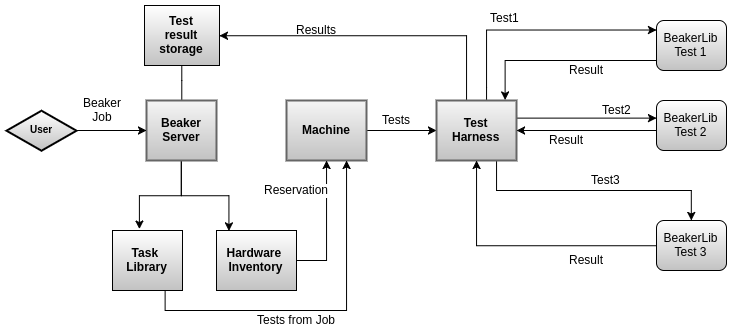
\includegraphics[width=\linewidth]{beaker_relations.png}
  \caption{Beaker relation to BeakerLib}
  \label{fig:beaker_relation}
\end{figure}




\chapter{BeakerLib}
This chapter takes a closer look on inner workings of BeakerLib, with focus on Journal feature.

\section{Important functions}
As stated earlier BeakerLib is shell-level library with functions that make writing and running tests easier as well as examining their results.
BeakerLib adds testing functions to \texttt{shell} functionality, so user can combine normal \texttt{shell} commands and constructions with helping functions which can make writing tests and examining their results easier. There is close to 80 of these functions (also known as rlCommands), descriptions of most used ones follows:
\begin{itemize}
\item \textbf{rlRun} - First argument of this function is any shell command, which is executed by rlRun. Second is an expected exit code of first argument, it can contain one or more codes. Third argument is a comment. BeakerLib logs \texttt{FAIL} or \texttt{PASS} if expected exit code differs or not from actual one respectively along with comment. This is most used and important function.
\item \textbf{rlPass} - Manual assertion and logging of \texttt{PASS}. Useful when in combination with if statement which user doesn't want to appear in logs but still wants to log its result. Reciprocal function \textbf{rlFail} exists as well.
\item \textbf{rlAssertExists} - Asserts whether file given as a first argument exists.
\item \textbf{rlAssertGrep} - Function logs \texttt{PASS} when pattern given as first argument matches in a file which a second argument. Optional flags are passed to \texttt{grep} and behave the same way.
\item \textbf{rlAssertRpm} - Function asserts \texttt{PASS} when package given as first argument is installed.  Optional arguments allow specifying particular version, release or arch of the package.
\item \textbf{rlAssertDiffer} - Asserts whether two files given as argument differ in their content. 
\end{itemize}
\section{Phases}
BeakerLib divides tests into logical groups called Phases. There are three basic types of phases:
\begin{itemize}
\item Setup - preparing conditions for the test (such as creating temporary files, starting needed services and so on)
\item Test - main phase for testing
\item Cleanup - reverting changes made by the test
\end{itemize}
This division helps when examining the result of test as it shows which phase causes fail, if any, in BeakerLib's output. Example test \ref{lst:test_example} shows how basic BeakerLib test looks.
\\
\begin{lstlisting}[style=beakerlib_bash,caption={BeakerLib basic test example},label={lst:test_example}]
# Include Beaker environment
. /usr/bin/rhts-environment.sh || exit 1
. /usr/share/beakerlib/beakerlib.sh || exit 1
# Start of Journal
rlJournalStart
    # Start of Setup Phase, creating temp directory where test will take place 
    rlPhaseStartSetup
        rlAssertRpm $PACKAGE
        rlRun "TmpDir=\$(mktemp -d)" 0 "Creating tmp directory"
        rlRun "pushd $TmpDir"
    rlPhaseEnd
   # Start of Test Phase, testing touch and ls commands
    rlPhaseStartTest
        rlRun "touch foo" 0 "Creating the foo test file"
        rlAssertExists "foo"
        rlRun "ls -l foo" 0 "Listing the foo test file"
    rlPhaseEnd
   # Statr of Cleanup phase, temp directory is deleted
    rlPhaseStartCleanup
        rlRun "popd"
        rlRun "rm -r $TmpDir" 0 "Removing tmp directory"
    rlPhaseEnd
rlJournalPrint
rlJournalEnd
\end{lstlisting}


\section{BeakerLib's output}
BeakerLib produces 3 kinds of outputs 2 files and terminal one. Files are saved into directory created for each individual test. If the test is run locally temporary directory is created on system with \texttt{mktepm} command. If run on Beaker unique \textbf{TESTID} is generated for each test. This TESTID serves as a name for test directory as well as identifier which Beaker later uses when connecting test results with correct test.

\subsection{journal.txt}
\textit{journal.txt} is a plain text file with human readable record of test's progress. After end of each phase, copy of the file is sent to Beaker for storage.

\subsection{Terminal output}
If the executed test is connected to an \texttt{interactive shell} the same BeakerLib's output is printed to terminal's standard output (\texttt{stdout}) as well as to journal.txt. However \texttt{shell's} output is colored for increased readability.  

\subsection{journal.xml}
Last output is XML\footnote{eXtensible Markup Language} file. This file is stripped off of commands' output, but core information (such as which commands were executed, whether they passed or failed and so on) is kept. Also metadata about the test run (time of execution, which component was tested and more) as well as information about the hardware and software test was run on are added. \textit{journal.xml} is sent back to Beaker same as \textit{journal.txt} where it is available for further processing by automated tools. It also serves as a source of information about current state of the test during its execution, for example whether there is currently an open phase or how many failed tests or phases there are so far.


\section{Analysis of slow performance}
It was reported that BeakerLib suffers performance problems when running long tests. Time of processing each rlCommand grew longer after many (several hundreds and more) were used. Analysis of library was problematic due to lack of documentation, complex structure and uncommented code, however it indicated that problem lies with generating \textit{journal.xml}. 

Python script \textit{journalling.py}, responsible for most of BeakerLib's output creation, is called after each rlCommand to log its result into \textit{journal.xml}. This isn't big problem with small test as the \textit{journal.xml} file takes up only a few kilobytes, however when the file takes up dozens or hundreds of kilobytes, loading the file from disk, parsing, adding a line of log and then saving the file back to the disk adds significantly more load to CPU\footnote{Central Processing Unit}. 

\chapter{Solution of Journaling problem}
This chapter describes proposed solutions to optimize Journaling problem.

\section{Change of xml parser}
XML parser is a program which can turn XML document into structured object in RAM\footnote{Random Access Memory}. Depending on implementation of the parses, that object is then easier to access by the program as it may provide methods to navigate the object and search it or potentially modify. 

Parsing of XML in BeakerLib is done by \textit{journalling.py} script by \texttt{Python} module \texttt{xml.dom.minidom}, which I decided to change to different one, to measure whether it will provide better performance. Because of reasons of backward compatibility to RHEL 5\footnote{Red Hat Enterprise Linux 5} which supports BeakerLib, the choice of XML parsers was limited to native modules of \texttt{Python 2.4.3}. Two additional XML parsers were present for given version.

\begin{itemize}
\item xml.sax -  [https://docs.python.org/2/library/xml.sax.html] <expand>
\item lxml - [http://lxml.de/] <expand>
\end{itemize}

I decided to implement \texttt{lxml} parser as it is supposed to be faster and less demanding on memory than \texttt{xml.dom.minidom} [http://lxml.de/performance.html].

\section{Change in calling journalling.py}
Next proposition to make BeakerLib faster is in a way \textit{journalling.py} is called. The assumption being that repeated parsing of XML document slows BeakerLib the most, reducing the number of times it was parsed was then the highest priority. 

\subsection{Queue file solution}
First solution is to create a new, temporary \texttt{queue file}, which will act as a buffer. rlCommands will behave as before apart from creating BeakerLib journals but instead they will write message into the queue file. This file will be read and processed only when necessary, that is at the end each phase, when journals are sent to Beaker.

\subsubsection{Disadvantages}
The way BeakerLib is designed now it in most cases expects some form of return value from \textit{journalling.py} immediately after adding a log to a journal. Performed logging either returns code indicating success of failure or \texttt{string} with information about the current state of test. This presents problem as there is no way how to communicate back these information when parsing is postponed. 

\subsection{Daemon-like solution}
Second solution is to rewrite \textit{journalling.py} script to have daemon-like behavior. That is to have it run as its own process throughout the whole time of test execution. The xml object will be stored in memory, and parsed as whole only at the beginning of journal creation and in case of restarting the test run (which happen when machine is rebooted).  

This way BeakerLib can receive response about current test state immediately while still keeping CPU load minimal. Daemon-like solution however brings different obstacles.

\subsubsection{Disadvantages}
An independent, potentially long running process daemon is more prone to unplanned events such as unexpected exit. This must be addressed by both daemon (to exit as safely as possible)  and by the rest of BeakerLib (to detect that daemon is no longer running and to behave accordingly). 

\subsubsection{Communication}
 Synchronous inter-process communication between running test and daemon has to be created for test to  inform which rlCommand is supposed to be logged and for daemon to respond with current state of XML document. I considered two options:

\begin{itemize}
\item Unix sockets  -  <expand>
\item Named pipes - Named pipes are device files. They allow inter-process communication by reading it and writing into is as if regular file, however under normal circumstances the read/write is a blocking operation. This means if one process opens pipe for reading, it will hang there until another process opens the pipe for writing. This feature can be used for synchronization of communication between processes. 
\end{itemize}

I chose to implement communication through Named pipes because of built-in synchronization.


\chapter{Implementation of proposed solutions}
Thi chapter describes how were proposed solutions implemented.

\section{Change of xml parser}
\section{Difference in parsers}
As mentioned before I chose to change original XML parser to \texttt{lxml}. Only changes in code were in file \textit{journalling.py} as it is only part of BeakerLib that directly works with journal's XML object. 
Most of the changes consisted in changing \texttt{xml.dom.minidom's} method for creating new XML element and assigning value into it.
Biggest difference between given parsers is that \texttt{lxml} does not provide many helping methods as \texttt{xml.dom.minidom} does.
For example in \texttt{lxml}  there is no method \texttt{getElementsByTagName()} to search XML object by a tag name. Instead of it \texttt{lxml} supports \texttt{xpath} [https://www.w3schools.com/xml/xpath\_intro.asp] syntax for searching the object.

\subsubsection{xpath}
xpath\footnote{XML Path Language} is part of XSLT\footnote{eXtensible Stylesheet Language Transformations} standart. It can used to navigate through elements and attributes in an XML document. <expand???>
\\
\\
Another example of difference is an approach for accessing element's children. While \texttt{xml.dom.minidom} has dedicated methods and attributes such as \texttt{hasChildNodes()} which returns \texttt{bool} value or \texttt{childNodes} which is a iterable attribute of element's children, \texttt{lxml} has more low level implementation. It treats elements as python lists so \texttt{hasChildNodes()} can be replaced with simple \texttt{len(element)}.
\\
\\
During changing of parsers I discovered and fixed some bugs present in current implementation of \textit{journalling.py}, such as wrong path when searching for used plugins. ??? asi nedava smysl
\\
\\
Because preliminary performance measurement showed slightly faster test execution, I decided to implement the rest of the proposed solutions with the parser.

\section{Queue file solution}
\section{Daemon-like solution}

\section{testing that my solution is the same}

\chapter{Performance measuring}
<Definition of performance measuring>

For performance measuring of BeakerLib I chose two kinds of tests in in two kinds of testing environments.

\section{Tests}

\subsection{Artificial tests}
First type of tests are artificial tests created by me with \texttt{beaker-wizard} to specifically target and measure performance of journaling modification I made. They consist mostly of commands that directly work with \texttt{journalling.py}. For example commands \textbf{rlLog} or \textbf{rlPhaseStart} and \textbf{rlPhaseEnd}. This way we can observe clear difference in performance without being affected by operations unrelated to journaling (executing actions that verify functionality of components in real tests). 

<description of artificial tests with links to Appendix>

\subsection{Real tests}
Second type are real tests used in Red Hat. These are examples of tests that have been reported to have bad performance with BeakerLib so I am testing them to see if my modifications have real life impact on performance.

<description of real tests>

\section{Testing Environment}

\subsection{Local}
First environment is local laptop for convenience and speed of execution. I measured  two parameters, time of execution of each test and memory usage during execution. Tests were run directly, without any harness and with these technical specifications. 

<table of tech specs>

\subsection{Remote in beaker}
Second round of testing was done to emulate real testing conditions and to verify that changes made to BeakerLib do not break functionality outside of controlled environment. Tests were run with the default test harness Beah. Only overall time of execution of each test was measured in remote testing.

<table of tech specs>

\section{Baseline measurements}
<results>


\section{Implemented optimizations}
<results>

\chapter{Conclusion}
Recap of results
\\
Future work


%=========================================================================
